\section*{Ora e sede}
13:30 Viale Morgagni
\section*{Invitati e presenti}
Committente PMango e Fornitori
\section*{Ordine del giorno}
\begin{enumerate}
\item Organizzazione fra fornitori
\item Aree PMango su cui lavorare
\item Notazioni per i Task
\end{enumerate}

\section*{Discussione}
\begin{enumerate}
\item Organizzazione fra fornitori: vantaggi e svantaggi di lavorare in competizione o cooperazione

\item Aree PMango su cui lavorare
\begin{itemize}

\item Generazione di Gif per 
	\begin{itemize}
		\item Gantt (aggiungere funzionalit\`a all'esistente)
		\item Wbs (nuovo tab)
		\item Tasknetworks (nuovo tab)
	\end{itemize}
\item Generazione di Pdf (con gli stessi punti espressi per la generazione gif.

\item Interfaccia utente per 
	\begin{itemize}
		\item Gantt (opzioni per le nuove funzionalit\`a)
		\item Wbs (opzioni di visualizzazione)
		\item Tasknetworks (opzioni di visualizzazione)
	\end{itemize}

\item  Documentazione (Manuale Utente) creando un manuale per le nuove funzionalit\`a

\item Test, Le nuove funzionalit\`a andranno testate bene

\item  Codice condiviso, per disegnare Wbs,Gantt e Tasknetworks ci sono API comuni da specializzare poi nei loro usi (pdf, gif)

\end{itemize}
\item Notazioni per i Task
\begin{itemize}
\item Gantt
	\begin{itemize}
		\item Opzione per disegnare la Wbs fino a livello N
		\item Riportare risorse, impegno...
		\item Riportare tempi completamento, attuale...
		\item Funzioni makepdf e addtoreport
		\item Colori e grafica carini
			\begin{figure}[h] 
				\centering 
				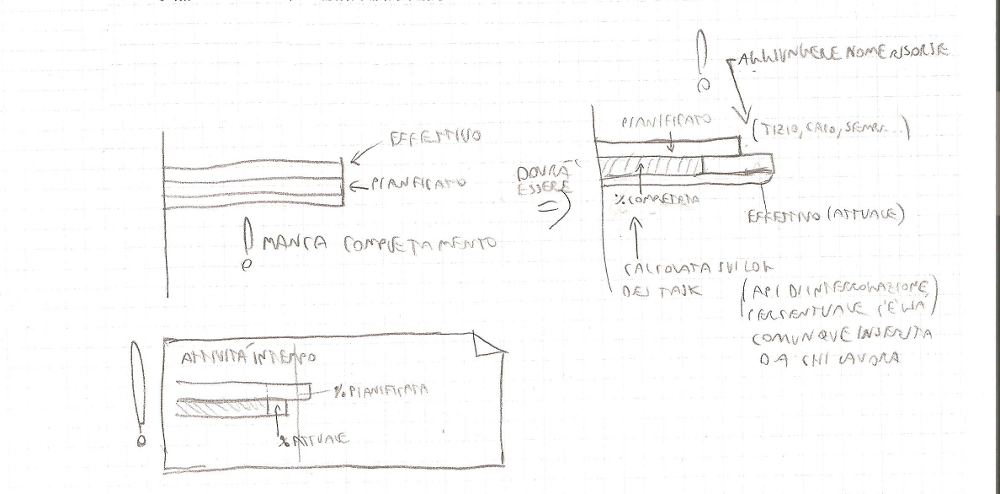
\includegraphics[width=1\textwidth]{gantt_draft.png} 
				\caption{gantt draft}
				\label{fig:firstAnalisys_GanttChart}			
			\end{figure}
	\end{itemize}

\item{WBS}
	\begin{figure}[h] 
				\centering 
				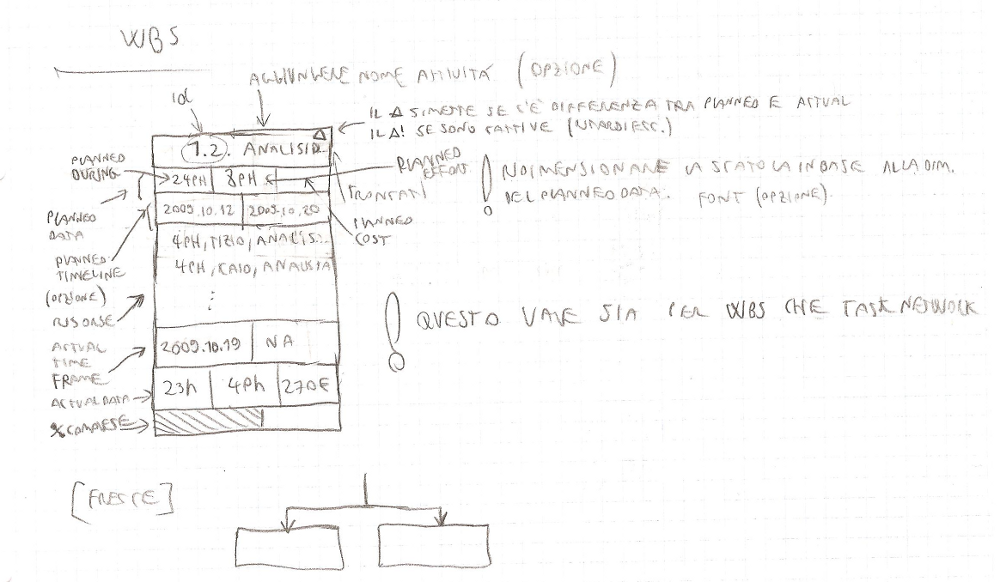
\includegraphics[width=1\textwidth]{wbs_draft.png} 
				\caption{wbs draft}
				\label{fig:firstAnalisys_WBSChart}			
			\end{figure}
\end{itemize}
\end{enumerate}

\newpage
\section*{Varie e eventuali}
Domande del team:
\begin{itemize}
\item Quali funzioni aggiungere al Gantt gi\`a presente?
Gi\`a affrontato nell'ordine del giorno
\item Come deve apparire il cpm?
Da definire meglio nei prossimi incontri
\item Cosa abbiamo a disposizione come moduli gi\`a sviluppati?
Use the code Luke!
\item Il Gantt deve comprendere le derivarables?
No, attualmente ci sono le milestones ma le deriverables non interessano
\item Si preferisce pi\`u informazioni o maggiore chiarezza visiva?
Bilanciare con le opzioni Gui cos\`i che sia l'utente a decidere
\end{itemize}

\section*{Chiusura della riunione}
Riunione chiusa alle 15.30
